Un'analisi cruciale che può essere eseguita su un dataset di traiettorie è sicuramente
la ricerca di oggetti che si muovono assieme.
Un \textit{co-movement} pattern~\cite{zheng2015trajectory} individua un gruppo di oggetti che si sono mossi assieme
per un certo tempo, l'apparteneza a tale gruppo è determinata solitamente dalla vicinanza nello
spazio.
La ricerca di questi pattern di movimento include diversi parametri che definiscono le
caratteristiche dei gruppi individuati. Varie tipologie di cluster sono state definite
in letteratura sulla base dell'adozione e configurazione di questi parametri.

Prima di scendere nel dettaglio, occorre definire gli elementi principali della ricerca.
Innanzitutto dato un dataset di traiettorie \(TR_{db} = \{tr_{1}, \ldots, tr_{n}\} \), da questo viene derivato il dataset
degli oggetti che hanno generato quelle traiettorie, \(O_{db} = \{ o_{1}, ldots, o_{m} \}, m <= n\)
e un dataset contenete tutti i possibili istanti temporali del primo dataset
\(T_{db} = \{t_{1}, ldots, t_{k}\} \).
In generale, nella ricerca di \textit{co-movement} pattern si ricerca un certo \(O = \{ o_{1}, ldots, o_{p} \}, O \subseteq O_{db} \)
tale che il corrispondente \(T = \{t_{1}, ldots, t_{j}\} T \subseteq T_{sb}\) goda di certe proprietà, come
ad esempio una lunghezza minima, oppure una continuità all'interno del tempo.
Due parametri comuni a tutti i pattern di movimento sono la \(m\), che individua una
dimensione minima per la dimensione di \(O\) e \(k\), limite inferiore al numero
di istanti temporali in cui il gruppo in questione è considerato vicino.

Il primo pattern di movimento individuabile alla luce dei vincoli appena espressi è
\textit{swarm}~\cite{li2010swarm}. In maniera informale, swarm ricerca gruppi di \(m\) oggetti che hanno viaggiato
assieme per almeno \(k\) istanti temporali senza porre alcun ulteriore vincolo.
Uno swarm può essere definito come segue:

\begin{definition}[Swarm]\label{definition:swarm}

  Una coppia \( \{ O, T \} \) si definisce swarm se:

  \begin{center}

    \(
      \begin{cases}
         \forall t \in T,\exists c \; s.t. \; O \in c \\
         |O| \geq m \\
         |T| \geq k

      \end{cases}
      \)

  \end{center}
\end{definition}

La~\cref{definition:swarm} formalizza i seguenti vincoli:
ad ogni istante di \(T\) gli oggetti di \(O\) devono appartenere a uno stesso cluster,
il gruppo deve essere poi rilevante dal punto di vista degli elementi (\(m\)) e del tempo trascorso
(\(k\)).
Per quanto riguarda il primo vincolo, è possibile utilizzare varie metriche per fare clustering
sulla dimensione spaziale del dataset, tuttavia l'algoritmo più utilizzato per la ricerca di swarm
è DBSCAN\@.


Il concetto di swarm può essere ulteriormente raffinato in quello di \textit{closed swarm}:
un closed swarm intuitivamente si definisce allo stesso modo di uno swarm, ma con l'ulteriore
vincolo di considerare la massima sequenza di istanti in cui gli oggetti dentro \(O\) risultano vicini
tra di loro (chiusura rispetto al tempo) oppure il numero massimo di oggetti dato un certo \(T\)(chiusura rispetto agli oggetti).
Formalmente, ciò è espresso nella~\cref{definition:closed-swarm}

\begin{definition}[Closed Swarm]\label{definition:closed-swarm}

  Una coppia \( \{ O, T \} \) si definisce closed-swarm se:

  \begin{center}

    \(
      \begin{cases}
         \{ O, T \} \; is \; swarm   \\
         \nexists O' \; s.t. \;  \{ O \cup O', T \} is swarm   \\
         \nexists T' \; s.t. \;  \{ O, T \cup T' \} is swarm
      \end{cases}
    \)

  \end{center}

\end{definition}

Com'è possibile vedere in~\cref{fig:chap-1:SwarmExample} (Fonte:~\cite{phan2016all}), la ricerca di swarm produce riconosce
il gruppo \( \{ o_{1}, o_{2}\} \) in quanto i due oggetti risultano avere viaggiato vicini per almeno
tre istanti temporali (\(t_{1}, t_{2}, t_{4}\)).

\begin{figure}
  \centering
  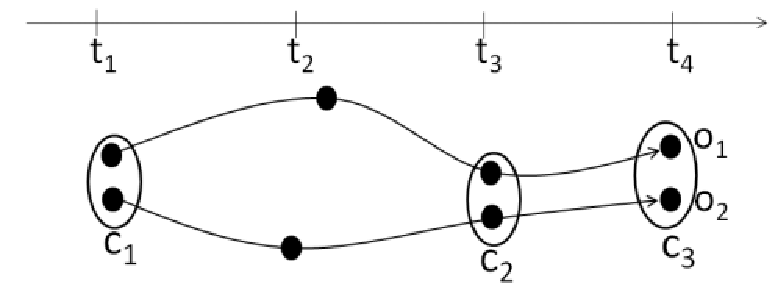
\includegraphics[scale=.8]{/sec-1/SwarmExample.pdf}
  \caption{Ricerca di Swarm su un dataset fissati \(m=2\) e \(k=3\)}%
  \label{fig:chap-1:SwarmExample}
\end{figure}


Entrambi i pattern appena presentati rilassano al massimo i vincoli sul tempo,
accettando gruppi aventi istanti temporali parecchio distanti gli uni dagli altri.
Un tipo di analisi che aggiunge un rigido vincolo sulla continuità degli istanti temporali è
la ricerca di \textit{convoy}~\cite{jeung2008convoy}: un convoy per definizione è un raggruppamento di oggetti \(O\) in cui
tutti gli istanti in \(T\) sono consecutivi, mantenendo i precedenti vincoli sulle dimensioni del
gruppo e sul tempo trascorso assieme.

\begin{definition}[Convoy]\label{definition:convoy}
  Una coppia \( \{ O, T \} \) si definisce convoy se:
  \begin{center}
    \(
      \begin{cases}
         \{ O, T \} \; is \; swarm   \\
      \forall t_{i} \in T, t_{i+1} = t_{i} + 1
      \end{cases}
    \)

  \end{center}
\end{definition}

Analogamente a quanto accade per swarm, anche convoy utilizza DBSCAN per determinare
la vicinanza o meno di due oggetti in base all'appartenenza a un certo cluster ad ogni
\(t_{i}\).
Qualora si voglia adottare un algoritmo non basato sulla densità per determinare la vicinanza, allora i
pattern individuati sono chiamati \textit{flock}~\cite{benkert2008reporting} pattern.
La~\cref{fig:chap-1:ConvoyExample} (Fonte:~\cite{phan2016all}) mostra un esempio di ricerca di convoy: fissati \(m=2\)
e \(k=3\), risulta come pattern valido \( \{ o_{1}, o_{2}\} \),
\( \{ o_{1}, o_{2}, o_{3}\} \) viene scartato in quanto non soddisfa il vincolo di continuità
sugli istanti temporali.

\begin{figure}
  \centering
  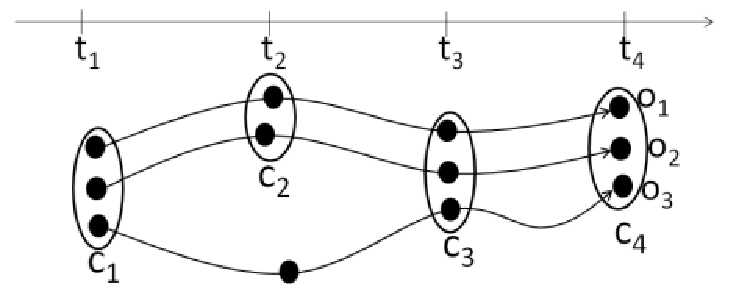
\includegraphics[scale=.8]{/sec-1/ConvoyExample.pdf}
  \caption{Ricerca di Convoy su un dataset fissati \(m=2\) e \(k=3\)}%
  \label{fig:chap-1:ConvoyExample}
\end{figure}

Convoy e Swarm rappresentano i due casi limiti per quanto riguarda la rigidità dei vincoli temporali,
Swarm rilassa totalmente la continuità mentre Convoy esige una rigidità assoluta nella sequenza
degli istanti temporali.
Una via di mezzo tra i due estremi è individuata nel pattern \textit{Group}~\cite{wang2006efficient}.
Un pattern group individua un insieme di convoy disgiunti relativi allo stesso gruppo di oggetti \(O\);
interpretando ogni convoy come un singolo punto temporale \(t_{s}\), un pattern group può essere visto come uno swarm
di convoy.
Ognuno dei singoli punti così individuati dovrà risultare come valido convoy, si definisce
il parametro \textit{l} come la lunghezza di istanti condivisi in ognuno dei punti individuati.

\begin{definition}[Group]\label{definition:group}
  Definito \(T_{s}\) come l'insieme degli istanti temporali generati dai singoli group,
  una coppia \( \{ O, T_{s} \} \) si definisce group se:
  \begin{center}
    \(
      \begin{cases}
         \{ O, T_{s} \} \; is \; swarm   \\
      \forall t_{si} \in T_{s}, \; |t_{s}| \geq l
      \end{cases}
    \)

  \end{center}
\end{definition}

Group introduce la possibilità di ricercare gruppi con una continuità rilassata, tuttavia
non pone nessun vincolo sul numero complessivo di istanti necessari per considerare
un pattern interessante.
Per integrare questo parametro, è stato definito il pattern \textit{Platoon}~\cite{li2015efficient}.
Questo approccio interpreta diversamente il valore di \textit{k} rispetto a quanto fatto in
group: se in quest'ultimo approccio \(k\) indicava il numero di convoy necessari per individuare
un raggruppamento valido, ora \(k\) indica il numero di istanti assoluti necessari per
un platoon valido.
In termini formali, il pattern platoon può essere definito come segue:

\begin{definition}[Platoon]\label{definition:platoon}
  Definito \(T_{s}\) come l'insieme degli istanti temporali generati dai singoli convoy,
  una coppia \( \{ O, T \} \) si definisce group se:
  \begin{center}
    \(
      \begin{cases}
         \{ O, T \} \; is \; swarm   \\
      \forall t_{si} \in T_{s}, \; |t_{s}| \geq l
      \end{cases}
    \)

  \end{center}
\end{definition}

Terminata l'esposizione dei principali pattern di co-movimento, la
~\cref{fig:chap-1:AllExample} (Fonte:~\cite{DBLP:journals/pvldb/FanZWT16}) mostra
quali sono le differenze, a parità di valori di \(m, k \) e \(l\), tra i diversi pattern di movimento.
Dalla figura in questione emergono chiaramente le differenze tra i gruppi individuati dai
vari pattern: ad esempio group riconosce \( \{ o_{3}, o_{4}, o_{5}\} \) negli istanti \( \{ 1, 2 \} \)
poiché la lunghezza di tale sottosequenza risulta uguale ad \(l\); platoon invece spezza
il raggruppamento in \( \{ o_{3}, o_{4} \}, \{ o_{4}, o_{5} \} \) poiché quest'ultimo non
avrebbe rispettato il vincolo sulla lunghezza minima degli istanti \(k\).

\begin{figure}
  \centering
  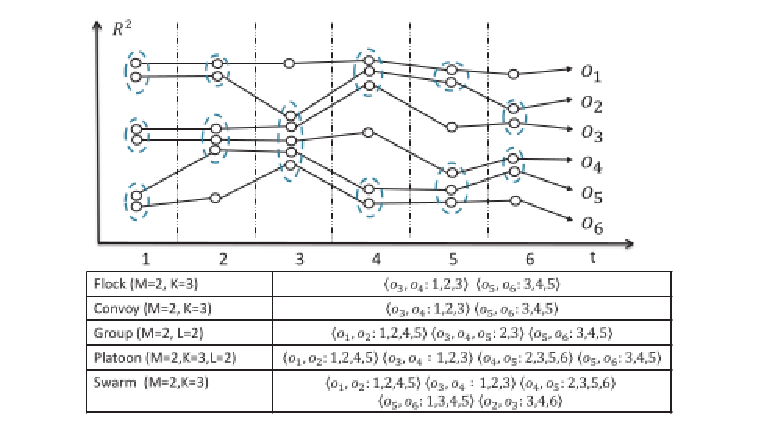
\includegraphics[scale=.8]{/sec-1/AllExamples.pdf}
  \caption{Ricerca dei principali pattern di movimento su un dataset fissati \(m=2\), \(k=3\) e \(l=2\)}%
  \label{fig:chap-1:AllExample}
\end{figure}
